% Options for packages loaded elsewhere
\PassOptionsToPackage{unicode}{hyperref}
\PassOptionsToPackage{hyphens}{url}
%
\documentclass[
]{article}
\usepackage{amsmath,amssymb}
\usepackage{iftex}
\ifPDFTeX
  \usepackage[T1]{fontenc}
  \usepackage[utf8]{inputenc}
  \usepackage{textcomp} % provide euro and other symbols
\else % if luatex or xetex
  \usepackage{unicode-math} % this also loads fontspec
  \defaultfontfeatures{Scale=MatchLowercase}
  \defaultfontfeatures[\rmfamily]{Ligatures=TeX,Scale=1}
\fi
\usepackage{lmodern}
\ifPDFTeX\else
  % xetex/luatex font selection
\fi
% Use upquote if available, for straight quotes in verbatim environments
\IfFileExists{upquote.sty}{\usepackage{upquote}}{}
\IfFileExists{microtype.sty}{% use microtype if available
  \usepackage[]{microtype}
  \UseMicrotypeSet[protrusion]{basicmath} % disable protrusion for tt fonts
}{}
\makeatletter
\@ifundefined{KOMAClassName}{% if non-KOMA class
  \IfFileExists{parskip.sty}{%
    \usepackage{parskip}
  }{% else
    \setlength{\parindent}{0pt}
    \setlength{\parskip}{6pt plus 2pt minus 1pt}}
}{% if KOMA class
  \KOMAoptions{parskip=half}}
\makeatother
\usepackage{xcolor}
\usepackage[margin=1in]{geometry}
\usepackage{color}
\usepackage{fancyvrb}
\newcommand{\VerbBar}{|}
\newcommand{\VERB}{\Verb[commandchars=\\\{\}]}
\DefineVerbatimEnvironment{Highlighting}{Verbatim}{commandchars=\\\{\}}
% Add ',fontsize=\small' for more characters per line
\usepackage{framed}
\definecolor{shadecolor}{RGB}{248,248,248}
\newenvironment{Shaded}{\begin{snugshade}}{\end{snugshade}}
\newcommand{\AlertTok}[1]{\textcolor[rgb]{0.94,0.16,0.16}{#1}}
\newcommand{\AnnotationTok}[1]{\textcolor[rgb]{0.56,0.35,0.01}{\textbf{\textit{#1}}}}
\newcommand{\AttributeTok}[1]{\textcolor[rgb]{0.13,0.29,0.53}{#1}}
\newcommand{\BaseNTok}[1]{\textcolor[rgb]{0.00,0.00,0.81}{#1}}
\newcommand{\BuiltInTok}[1]{#1}
\newcommand{\CharTok}[1]{\textcolor[rgb]{0.31,0.60,0.02}{#1}}
\newcommand{\CommentTok}[1]{\textcolor[rgb]{0.56,0.35,0.01}{\textit{#1}}}
\newcommand{\CommentVarTok}[1]{\textcolor[rgb]{0.56,0.35,0.01}{\textbf{\textit{#1}}}}
\newcommand{\ConstantTok}[1]{\textcolor[rgb]{0.56,0.35,0.01}{#1}}
\newcommand{\ControlFlowTok}[1]{\textcolor[rgb]{0.13,0.29,0.53}{\textbf{#1}}}
\newcommand{\DataTypeTok}[1]{\textcolor[rgb]{0.13,0.29,0.53}{#1}}
\newcommand{\DecValTok}[1]{\textcolor[rgb]{0.00,0.00,0.81}{#1}}
\newcommand{\DocumentationTok}[1]{\textcolor[rgb]{0.56,0.35,0.01}{\textbf{\textit{#1}}}}
\newcommand{\ErrorTok}[1]{\textcolor[rgb]{0.64,0.00,0.00}{\textbf{#1}}}
\newcommand{\ExtensionTok}[1]{#1}
\newcommand{\FloatTok}[1]{\textcolor[rgb]{0.00,0.00,0.81}{#1}}
\newcommand{\FunctionTok}[1]{\textcolor[rgb]{0.13,0.29,0.53}{\textbf{#1}}}
\newcommand{\ImportTok}[1]{#1}
\newcommand{\InformationTok}[1]{\textcolor[rgb]{0.56,0.35,0.01}{\textbf{\textit{#1}}}}
\newcommand{\KeywordTok}[1]{\textcolor[rgb]{0.13,0.29,0.53}{\textbf{#1}}}
\newcommand{\NormalTok}[1]{#1}
\newcommand{\OperatorTok}[1]{\textcolor[rgb]{0.81,0.36,0.00}{\textbf{#1}}}
\newcommand{\OtherTok}[1]{\textcolor[rgb]{0.56,0.35,0.01}{#1}}
\newcommand{\PreprocessorTok}[1]{\textcolor[rgb]{0.56,0.35,0.01}{\textit{#1}}}
\newcommand{\RegionMarkerTok}[1]{#1}
\newcommand{\SpecialCharTok}[1]{\textcolor[rgb]{0.81,0.36,0.00}{\textbf{#1}}}
\newcommand{\SpecialStringTok}[1]{\textcolor[rgb]{0.31,0.60,0.02}{#1}}
\newcommand{\StringTok}[1]{\textcolor[rgb]{0.31,0.60,0.02}{#1}}
\newcommand{\VariableTok}[1]{\textcolor[rgb]{0.00,0.00,0.00}{#1}}
\newcommand{\VerbatimStringTok}[1]{\textcolor[rgb]{0.31,0.60,0.02}{#1}}
\newcommand{\WarningTok}[1]{\textcolor[rgb]{0.56,0.35,0.01}{\textbf{\textit{#1}}}}
\usepackage{graphicx}
\makeatletter
\newsavebox\pandoc@box
\newcommand*\pandocbounded[1]{% scales image to fit in text height/width
  \sbox\pandoc@box{#1}%
  \Gscale@div\@tempa{\textheight}{\dimexpr\ht\pandoc@box+\dp\pandoc@box\relax}%
  \Gscale@div\@tempb{\linewidth}{\wd\pandoc@box}%
  \ifdim\@tempb\p@<\@tempa\p@\let\@tempa\@tempb\fi% select the smaller of both
  \ifdim\@tempa\p@<\p@\scalebox{\@tempa}{\usebox\pandoc@box}%
  \else\usebox{\pandoc@box}%
  \fi%
}
% Set default figure placement to htbp
\def\fps@figure{htbp}
\makeatother
\setlength{\emergencystretch}{3em} % prevent overfull lines
\providecommand{\tightlist}{%
  \setlength{\itemsep}{0pt}\setlength{\parskip}{0pt}}
\setcounter{secnumdepth}{5}
\ifLuaTeX
\usepackage[bidi=basic]{babel}
\else
\usepackage[bidi=default]{babel}
\fi
\babelprovide[main,import]{spanish}
% get rid of language-specific shorthands (see #6817):
\let\LanguageShortHands\languageshorthands
\def\languageshorthands#1{}
\usepackage{bookmark}
\IfFileExists{xurl.sty}{\usepackage{xurl}}{} % add URL line breaks if available
\urlstyle{same}
\hypersetup{
  pdftitle={Análisis del Play-Delay en Netflix},
  pdfauthor={Luz Alba Posse \& Martina Monastra},
  pdflang={es},
  hidelinks,
  pdfcreator={LaTeX via pandoc}}

\title{Análisis del Play-Delay en Netflix}
\author{Luz Alba Posse \& Martina Monastra}
\date{2024-10-19}

\begin{document}
\maketitle

{
\setcounter{tocdepth}{2}
\tableofcontents
}
\section{Datos Históricos}\label{datos-histuxf3ricos}

\subsection{Histograma}\label{histograma}

Para evaluar los datos históricos, calculamos la media y la varianza del
play-delay y graficamos un histograma para verificar la forma de la
distribución.

\begin{Shaded}
\begin{Highlighting}[]
\NormalTok{historical\_data }\OtherTok{\textless{}{-}} \FunctionTok{read.csv}\NormalTok{(}\StringTok{"datos\_historicos.csv"}\NormalTok{)}

\NormalTok{mean\_historical }\OtherTok{\textless{}{-}} \FunctionTok{mean}\NormalTok{(historical\_data}\SpecialCharTok{$}\NormalTok{play.delay)}
\NormalTok{variance\_historical }\OtherTok{\textless{}{-}} \FunctionTok{var}\NormalTok{(historical\_data}\SpecialCharTok{$}\NormalTok{play.delay)}

\NormalTok{mean\_historical}
\end{Highlighting}
\end{Shaded}

\begin{verbatim}
## [1] 42.17103
\end{verbatim}

\begin{Shaded}
\begin{Highlighting}[]
\NormalTok{variance\_historical}
\end{Highlighting}
\end{Shaded}

\begin{verbatim}
## [1] 54.30905
\end{verbatim}

\begin{Shaded}
\begin{Highlighting}[]
\FunctionTok{hist}\NormalTok{(historical\_data}\SpecialCharTok{$}\NormalTok{play.delay, }
     \AttributeTok{breaks =} \DecValTok{30}\NormalTok{, }
     \AttributeTok{main =} \StringTok{"Play{-}Delay Histórico"}\NormalTok{, }
     \AttributeTok{xlab =} \StringTok{"Play{-}Delay"}\NormalTok{, }
     \AttributeTok{col =} \StringTok{"blue"}\NormalTok{, }
     \AttributeTok{border =} \StringTok{"black"}\NormalTok{)}

\FunctionTok{abline}\NormalTok{(}\AttributeTok{v =}\NormalTok{ mean\_historical, }\AttributeTok{col =} \StringTok{"red"}\NormalTok{, }\AttributeTok{lwd =} \DecValTok{2}\NormalTok{, }\AttributeTok{lty =} \DecValTok{2}\NormalTok{)}
\end{Highlighting}
\end{Shaded}

\pandocbounded{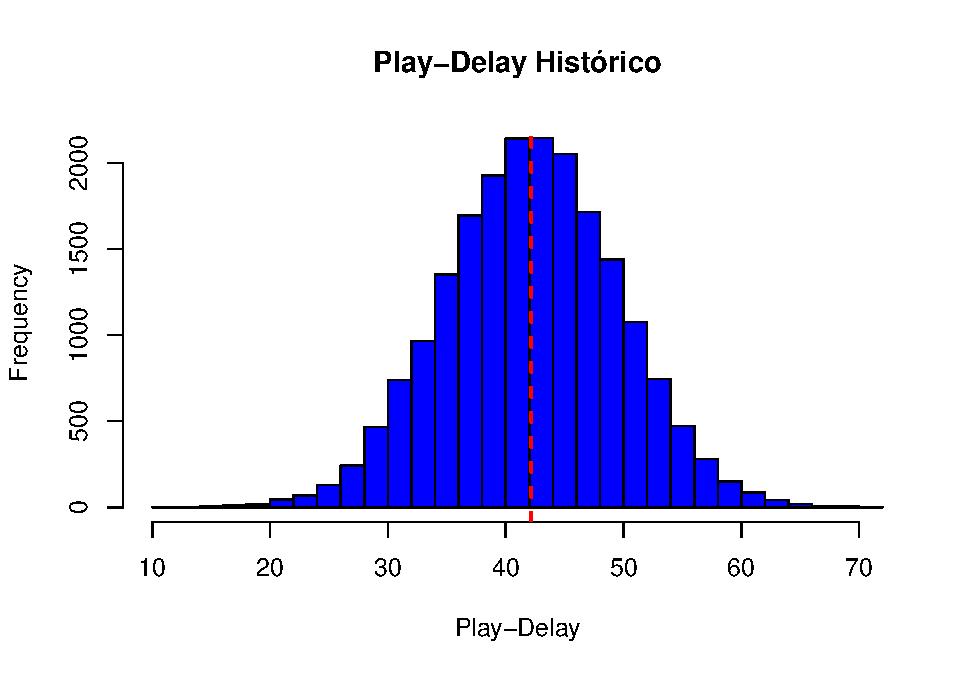
\includegraphics[keepaspectratio]{trabajo_practico_files/figure-latex/cargar-datos-1.pdf}}

Como bien vemos en el gráfico, los datos parecen distribuirse de forma
normal, con una media de 42.17103 y una varianza de 54.30905.

\section{Grupo de Prueba}\label{grupo-de-prueba}

\subsection{Estimación de la Media (µ) del Play-Delay para la Nueva
Versión}\label{estimaciuxf3n-de-la-media-uxb5-del-play-delay-para-la-nueva-versiuxf3n}

Se estima la esperanza del ``play-delay'' para los nuevos 200 usuarios
(grupo de prueba). La media se utiliza como estimador de µ,
representando el ``play-delay'' medio en la nueva versión de la
plataforma.

\begin{Shaded}
\begin{Highlighting}[]
\NormalTok{new\_data }\OtherTok{\textless{}{-}} \FunctionTok{read.csv}\NormalTok{(}\StringTok{"datos\_nuevos.csv"}\NormalTok{)}

\NormalTok{mean\_new }\OtherTok{\textless{}{-}} \FunctionTok{mean}\NormalTok{(new\_data}\SpecialCharTok{$}\NormalTok{play.delay)}

\NormalTok{mean\_new}
\end{Highlighting}
\end{Shaded}

\begin{verbatim}
## [1] 42.9895
\end{verbatim}

\section{Construir el test}\label{construir-el-test}

\subsection{Formulación de la
Hipotesis}\label{formulaciuxf3n-de-la-hipotesis}

\begin{itemize}
\tightlist
\item
  Hipótesis Nula (\(H_0\)): El play-delay promedio con la nueva versión
  es igual al de la versión anterior. \(μ = μ_0\), donde \(μ_0\) es la
  media del play-delay histórico.
\item
  Hipótesis Alternativa (\(H_1\)): El play-delay promedio con la nueva
  versión es mayor al de la versión anterior. Esto implica que
  \(μ > μ_0\)
\end{itemize}

Entonces, vamos a rechazar H\_0 solo si la nueva versión empeora
(aumenta) el play-delay.

El estadístico que utilizaremos es el Z para muestras grandes, ya que
asumimos que el play-delay tiene una distribución normal y conocemos la
vairanza de los datos históricos. Entonces:

\(Z = \frac{\bar{X} - \mu_0}{\frac{\sigma_0}{\sqrt{n}}}\)

\subsection{\texorpdfstring{Región de Rechazo para
\(\alpha = 0.05\)}{Región de Rechazo para \textbackslash alpha = 0.05}}\label{regiuxf3n-de-rechazo-para-alpha-0.05}

El nivel de significancia \(\alpha\) es 0.05. El valor crítico
\(Z_{0.05}\) se obtiene de la tabla de distribución normal, que es
\textbf{1.645}.

La \textbf{región de rechazo} es entonces: \[
Z > 1.645
\]

Si el valor calculado de \(Z\) es mayor que 1.645, rechazamos \(H_0\) y
concluimos que la actualización aumenta el play-delay.

\section{Usar el test}\label{usar-el-test}

\subsection{Decisión basada en las 200 nuevas
observaciones}\label{decisiuxf3n-basada-en-las-200-nuevas-observaciones}

Calculamos el estadístico \(Z\) utilizando los datos de los 200 usuarios
de prueba y lo comparamos con el valor crítico para un nivel de
significancia \(\alpha = 0.05\).

\begin{Shaded}
\begin{Highlighting}[]
\CommentTok{\# Parámetros}
\NormalTok{mu\_0 }\OtherTok{\textless{}{-}}\NormalTok{ mean\_historical }
\NormalTok{sigma\_0 }\OtherTok{\textless{}{-}} \FunctionTok{sqrt}\NormalTok{(variance\_historical) }
\NormalTok{n }\OtherTok{\textless{}{-}} \DecValTok{200} 

\CommentTok{\# Estadístico Z}
\NormalTok{Z }\OtherTok{\textless{}{-}}\NormalTok{ (mean\_new }\SpecialCharTok{{-}}\NormalTok{ mu\_0) }\SpecialCharTok{/}\NormalTok{ (sigma\_0 }\SpecialCharTok{/} \FunctionTok{sqrt}\NormalTok{(n))}

\NormalTok{Z}
\end{Highlighting}
\end{Shaded}

\begin{verbatim}
## [1] 1.570643
\end{verbatim}

El valor del estadístico \(Z\) obtenido es \textbf{1.5706434}.

El valor crítico para \(\alpha = 0.05\) es \textbf{1.645}. Si el valor
de \(Z\) es mayor que este valor crítico, rechazamos la hipótesis nula
\(H_0\), concluyendo que la actualización incrementa el ``play-delay''.
Si \(Z\) es menor o igual a 1.645, no rechazamos \(H_0\).

\begin{Shaded}
\begin{Highlighting}[]
\CommentTok{\# Valor crítico para alpha = 0.05}
\NormalTok{Z\_critico }\OtherTok{\textless{}{-}} \FunctionTok{qnorm}\NormalTok{(}\FloatTok{0.95}\NormalTok{)}

\CommentTok{\# Comparar Z con el valor crítico}
\ControlFlowTok{if}\NormalTok{ (Z }\SpecialCharTok{\textgreater{}}\NormalTok{ Z\_critico) \{}
\NormalTok{  decision }\OtherTok{\textless{}{-}} \StringTok{"Rechazamos H0: La actualización aumenta el play{-}delay."}
\NormalTok{\} }\ControlFlowTok{else}\NormalTok{ \{}
\NormalTok{  decision }\OtherTok{\textless{}{-}} \StringTok{"No rechazamos H0: No hay evidencia suficiente."}
\NormalTok{\}}

\NormalTok{decision}
\end{Highlighting}
\end{Shaded}

\begin{verbatim}
## [1] "No rechazamos H0: No hay evidencia suficiente."
\end{verbatim}

Dado que el valor del estadístico \(Z = 1.5706434\) es menor que el
valor crítico \(Z_{0.05} = 1.645\), \textbf{no rechazamos la hipótesis
nula \(H_0\)}. Por lo tanto, no tenemos evidencia suficiente para
concluir que la nueva versión aumente el play-delay, y \textbf{no es
necesario enviar el código a revisión}.

\subsection{\texorpdfstring{Regiones de rechazo para otros valores de
\(\alpha\)}{Regiones de rechazo para otros valores de \textbackslash alpha}}\label{regiones-de-rechazo-para-otros-valores-de-alpha}

El valor de \(\alpha\) determina qué tan estrictos somos al rechazar
\(H_0\). Entonces, a medida que aumentamos \(\alpha\), la región de
rechazo se vuelve más amplia, lo que implica que será más fácil rechazar
\(H_0\). A continuación, analizamos la región de rechazo para otros
valores de \(\alpha\), como 0.01 y 0.1, y comparamos las decisiones.

\begin{Shaded}
\begin{Highlighting}[]
\CommentTok{\# Calcular valores críticos para diferentes alphas}
\NormalTok{Z\_critico\_01 }\OtherTok{\textless{}{-}} \FunctionTok{qnorm}\NormalTok{(}\FloatTok{0.99}\NormalTok{)  }\CommentTok{\# para alpha = 0.01}
\NormalTok{Z\_critico\_10 }\OtherTok{\textless{}{-}} \FunctionTok{qnorm}\NormalTok{(}\FloatTok{0.90}\NormalTok{)  }\CommentTok{\# para alpha = 0.1}

\CommentTok{\# Comparar Z con los valores críticos}
\ControlFlowTok{if}\NormalTok{ (Z }\SpecialCharTok{\textgreater{}}\NormalTok{ Z\_critico\_01) \{}
\NormalTok{  decision\_01 }\OtherTok{\textless{}{-}} \StringTok{"Rechazamos H0 para alpha = 0.01"}
\NormalTok{\} }\ControlFlowTok{else}\NormalTok{ \{}
\NormalTok{  decision\_01 }\OtherTok{\textless{}{-}} \StringTok{"No rechazamos H0 para alpha = 0.01"}
\NormalTok{\}}

\ControlFlowTok{if}\NormalTok{ (Z }\SpecialCharTok{\textgreater{}}\NormalTok{ Z\_critico\_10) \{}
\NormalTok{  decision\_10 }\OtherTok{\textless{}{-}} \StringTok{"Rechazamos H0 para alpha = 0.1"}
\NormalTok{\} }\ControlFlowTok{else}\NormalTok{ \{}
\NormalTok{  decision\_10 }\OtherTok{\textless{}{-}} \StringTok{"No rechazamos H0 para alpha = 0.1"}
\NormalTok{\}}

\NormalTok{decision\_01}
\end{Highlighting}
\end{Shaded}

\begin{verbatim}
## [1] "No rechazamos H0 para alpha = 0.01"
\end{verbatim}

\begin{Shaded}
\begin{Highlighting}[]
\NormalTok{decision\_10}
\end{Highlighting}
\end{Shaded}

\begin{verbatim}
## [1] "Rechazamos H0 para alpha = 0.1"
\end{verbatim}

Para un nivel de significancia \(\alpha = 0.01\), el valor crítico es
más alto (\(Z = 2.33\)), lo que hace más difícil rechazar \(H_0\). En
este caso, la decisión es \textbf{No rechazamos H0 para alpha = 0.01}.

Para \(\alpha = 0.1\), el valor crítico es más bajo (\(Z = 1.28\)), lo
que facilita rechazar \(H_0\). En este caso, la decisión es
\textbf{Rechazamos H0 para alpha = 0.1}.

Entonces, que concluimos con esto?

\begin{itemize}
\tightlist
\item
  \textbf{Para \(\alpha = 0.05\)}: No rechazamos \(H_0\) \(\rightarrow\)
  no hay evidencia suficiente para afirmar que la actualización aumenta
  el play-delay, por lo que no es necesario enviar el código a revisión.
\item
  \textbf{Para \(\alpha = 0.01\)}: Somos más estrictos, y la decisión es
  no rechazar \(H_0\).
\item
  \textbf{Para \(\alpha = 0.1\)}: Somos menos estrictos y estamos más
  dispuestos a rechazar \(H_0\).
\end{itemize}

\subsection{\texorpdfstring{Evaluar la decisión para diferentes valores
de
\(\alpha\)}{Evaluar la decisión para diferentes valores de \textbackslash alpha}}\label{evaluar-la-decisiuxf3n-para-diferentes-valores-de-alpha}

Vamos a evaluar la decisión del test para
\(\alpha = 0.01, 0.02, 0.03, \ldots, 0.10\). Básicamente, calculamos el
valor crítico para cada \(\alpha\) y vemos si rechazamos \(H_0\) o no.

\begin{Shaded}
\begin{Highlighting}[]
\CommentTok{\# Definir los diferentes valores de alpha}
\NormalTok{alphas }\OtherTok{\textless{}{-}} \FunctionTok{seq}\NormalTok{(}\FloatTok{0.01}\NormalTok{, }\FloatTok{0.10}\NormalTok{, }\AttributeTok{by =} \FloatTok{0.01}\NormalTok{)}

\CommentTok{\# Crear un dataframe para almacenar los resultados}
\NormalTok{resultados\_alpha }\OtherTok{\textless{}{-}} \FunctionTok{data.frame}\NormalTok{(}\AttributeTok{alpha =}\NormalTok{ alphas, }\AttributeTok{Z\_critico =} \ConstantTok{NA}\NormalTok{, }\AttributeTok{decision =} \ConstantTok{NA}\NormalTok{)}

\CommentTok{\# Evaluar el test para cada alpha}
\ControlFlowTok{for}\NormalTok{ (i }\ControlFlowTok{in} \DecValTok{1}\SpecialCharTok{:}\FunctionTok{length}\NormalTok{(alphas)) \{}
\NormalTok{  Z\_critico\_alpha }\OtherTok{\textless{}{-}} \FunctionTok{qnorm}\NormalTok{(}\DecValTok{1} \SpecialCharTok{{-}}\NormalTok{ alphas[i])}
\NormalTok{  decision\_alpha }\OtherTok{\textless{}{-}} \FunctionTok{ifelse}\NormalTok{(Z }\SpecialCharTok{\textgreater{}}\NormalTok{ Z\_critico\_alpha, }\StringTok{"Rechazamos H0"}\NormalTok{, }\StringTok{"No rechazamos H0"}\NormalTok{)}
  
  \CommentTok{\# Almacenar los resultados}
\NormalTok{  resultados\_alpha}\SpecialCharTok{$}\NormalTok{Z\_critico[i] }\OtherTok{\textless{}{-}}\NormalTok{ Z\_critico\_alpha}
\NormalTok{  resultados\_alpha}\SpecialCharTok{$}\NormalTok{decision[i] }\OtherTok{\textless{}{-}}\NormalTok{ decision\_alpha}
\NormalTok{\}}

\CommentTok{\# Mostrar los resultados}
\NormalTok{resultados\_alpha}
\end{Highlighting}
\end{Shaded}

\begin{verbatim}
##    alpha Z_critico         decision
## 1   0.01  2.326348 No rechazamos H0
## 2   0.02  2.053749 No rechazamos H0
## 3   0.03  1.880794 No rechazamos H0
## 4   0.04  1.750686 No rechazamos H0
## 5   0.05  1.644854 No rechazamos H0
## 6   0.06  1.554774    Rechazamos H0
## 7   0.07  1.475791    Rechazamos H0
## 8   0.08  1.405072    Rechazamos H0
## 9   0.09  1.340755    Rechazamos H0
## 10  0.10  1.281552    Rechazamos H0
\end{verbatim}

\subsection{\texorpdfstring{Encontrar el valor mínimo de \(\alpha\) para
rechazar
\(H_0\)}{Encontrar el valor mínimo de \textbackslash alpha para rechazar H\_0}}\label{encontrar-el-valor-muxednimo-de-alpha-para-rechazar-h_0}

Para calcular el p-valor, usamos la función acumulativa de la
distribución normal estándar \(P(Z \geq z)\).

\begin{Shaded}
\begin{Highlighting}[]
\NormalTok{p\_valor }\OtherTok{\textless{}{-}} \DecValTok{1} \SpecialCharTok{{-}} \FunctionTok{pnorm}\NormalTok{(Z)}

\NormalTok{p\_valor}
\end{Highlighting}
\end{Shaded}

\begin{verbatim}
## [1] 0.05813275
\end{verbatim}

Entonces, interpretamos que:

\begin{itemize}
\tightlist
\item
  Si el p-valor es muy pequeño, entonces es poco probable observar un
  valor como el de \(Z\) si \(H_0\) fuera verdadera. Esto sugiere que
  deberíamos rechazar \(H_0\).
\item
  En el contexto del problema, el p-valor nos indica cuán fuerte es la
  evidencia de que la nueva actualización aumenta el play-delay. Un
  p-valor bajo significaría que es muy probable que la actualización
  esté afectando negativamente la experiencia del usuario.
\end{itemize}

\section{Simulaciones del Error Tipo
1}\label{simulaciones-del-error-tipo-1}

\subsection{\texorpdfstring{Simulación de una muestra bajo
\(H_0\)}{Simulación de una muestra bajo H\_0}}\label{simulaciuxf3n-de-una-muestra-bajo-h_0}

Asumimos que \(H_0\) es verdadera y simulamos una nueva muestra de 200
observaciones, aplicamos el test y tomamos una decisión.

\begin{Shaded}
\begin{Highlighting}[]
\CommentTok{\# Parámetros}
\NormalTok{n }\OtherTok{\textless{}{-}} \DecValTok{200}
\NormalTok{mu\_0 }\OtherTok{\textless{}{-}}\NormalTok{ mean\_historical}
\NormalTok{sigma\_0 }\OtherTok{\textless{}{-}} \FunctionTok{sqrt}\NormalTok{(variance\_historical)}

\CommentTok{\# Simular una muestra}
\FunctionTok{set.seed}\NormalTok{(}\DecValTok{123}\NormalTok{)}
\NormalTok{muestra\_simulada }\OtherTok{\textless{}{-}} \FunctionTok{rnorm}\NormalTok{(n, }\AttributeTok{mean =}\NormalTok{ mu\_0, }\AttributeTok{sd =}\NormalTok{ sigma\_0)}

\CommentTok{\# Calcular el estadístico Z}
\NormalTok{media\_simulada }\OtherTok{\textless{}{-}} \FunctionTok{mean}\NormalTok{(muestra\_simulada)}
\NormalTok{Z\_simulado }\OtherTok{\textless{}{-}}\NormalTok{ (media\_simulada }\SpecialCharTok{{-}}\NormalTok{ mu\_0) }\SpecialCharTok{/}\NormalTok{ (sigma\_0 }\SpecialCharTok{/} \FunctionTok{sqrt}\NormalTok{(n))}

\CommentTok{\# Valor crítico y decisi��n}
\NormalTok{Z\_critico }\OtherTok{\textless{}{-}} \FunctionTok{qnorm}\NormalTok{(}\FloatTok{0.95}\NormalTok{)}
\ControlFlowTok{if}\NormalTok{ (Z\_simulado }\SpecialCharTok{\textgreater{}}\NormalTok{ Z\_critico) \{}
\NormalTok{  decision\_simulada }\OtherTok{\textless{}{-}} \StringTok{"Rechazamos H0"}
\NormalTok{\} }\ControlFlowTok{else}\NormalTok{ \{}
\NormalTok{  decision\_simulada }\OtherTok{\textless{}{-}} \StringTok{"No rechazamos H0"}
\NormalTok{\}}

\CommentTok{\# Mostrar el estadístico Z y la decisión}
\NormalTok{Z\_simulado}
\end{Highlighting}
\end{Shaded}

\begin{verbatim}
## [1] -0.1212044
\end{verbatim}

\begin{Shaded}
\begin{Highlighting}[]
\NormalTok{decision\_simulada}
\end{Highlighting}
\end{Shaded}

\begin{verbatim}
## [1] "No rechazamos H0"
\end{verbatim}

\subsection{Simulación de 10,000
muestras}\label{simulaciuxf3n-de-10000-muestras}

Repetimos el procedimiento anterior 10,000 veces para calcular qué
porcentaje de estas rechazamos \(H_0\), obteniendo una estimación del
error de tipo 1.

\begin{Shaded}
\begin{Highlighting}[]
\CommentTok{\# Parámetros}
\NormalTok{R }\OtherTok{\textless{}{-}} \DecValTok{10000}
\NormalTok{rechazos\_H0 }\OtherTok{\textless{}{-}} \DecValTok{0}

\CommentTok{\# Simulación de R muestras}
\FunctionTok{set.seed}\NormalTok{(}\DecValTok{123}\NormalTok{)}
\ControlFlowTok{for}\NormalTok{ (i }\ControlFlowTok{in} \DecValTok{1}\SpecialCharTok{:}\NormalTok{R) \{}
\NormalTok{  muestra }\OtherTok{\textless{}{-}} \FunctionTok{rnorm}\NormalTok{(n, }\AttributeTok{mean =}\NormalTok{ mu\_0, }\AttributeTok{sd =}\NormalTok{ sigma\_0)}
\NormalTok{  media\_muestra }\OtherTok{\textless{}{-}} \FunctionTok{mean}\NormalTok{(muestra)}
\NormalTok{  Z\_muestra }\OtherTok{\textless{}{-}}\NormalTok{ (media\_muestra }\SpecialCharTok{{-}}\NormalTok{ mu\_0) }\SpecialCharTok{/}\NormalTok{ (sigma\_0 }\SpecialCharTok{/} \FunctionTok{sqrt}\NormalTok{(n))}
  
  \ControlFlowTok{if}\NormalTok{ (Z\_muestra }\SpecialCharTok{\textgreater{}}\NormalTok{ Z\_critico) \{}
\NormalTok{    rechazos\_H0 }\OtherTok{\textless{}{-}}\NormalTok{ rechazos\_H0 }\SpecialCharTok{+} \DecValTok{1}
\NormalTok{  \}}
\NormalTok{\}}

\CommentTok{\# Calcular el porcentaje de rechazos}
\NormalTok{porcentaje\_rechazos }\OtherTok{\textless{}{-}}\NormalTok{ (rechazos\_H0 }\SpecialCharTok{/}\NormalTok{ R) }\SpecialCharTok{*} \DecValTok{100}
\NormalTok{porcentaje\_rechazos}
\end{Highlighting}
\end{Shaded}

\begin{verbatim}
## [1] 4.95
\end{verbatim}

El porcentaje de veces que rechazamos \(H_0\) es \textbf{4.95\%}.

\subsection{\texorpdfstring{Interpretación Teórica de
\(\alpha\)}{Interpretación Teórica de \textbackslash alpha}}\label{interpretaciuxf3n-teuxf3rica-de-alpha}

El nivel de significancia \(\alpha\) representa la probabilidad de
cometer un error de tipo 1, es decir, rechazar \(H_0\) cuando en
realidad es verdadera. En nuestro caso, con \(\alpha = 0.05\), esperamos
que aproximadamente el 5\% de las veces cometamos este error al realizar
muchas pruebas. Lo que es consistente con el resultado obtenido en la
simulación anterior.

\end{document}
